\subsection{Evaluating Performance Comparison Results}

%\textbf{COHEN: How did the program performance compare to its selected standard?} 
%\textbf{Did the program demonstrate good performance?}
%\textbf{Is the programs performance different from predictions?} 
%\textbf{Did you learn what you wanted from the experiments?}

The best route set, having four routes, constructed by the proposed algorithm (SSO) is presented in Table \vref{table:performanceComparison_bestRouteSet4} and illustrated in Fig. \vref{fig:bestRouteSet4}. The best route set, having four routes, constructed by a plain ACO implementation is found in Table \vref{table:performanceComparison_bestRouteSet4_ACO}. The best, worst, average, median produced results with the standard deviation can be found in Appendix \ref{appendixC}, Table \vref{table:performanceComparison_ACOFull}. 

As one can see in Table \vref{table:performanceComparison_ACOSSOBEST}, the SSO performs overall better than the plain ACO implementation concerning the performance criteria. In ACO, compared to SSO, the ants do not possess memory, which is a feature that enables ants to ``remember'' nodes visited. This feature makes the ants favor nodes not visited over nodes already visited within the same route set, because Constraint \vref{itm:criteriaConnectedGraph} states that the produced route network must be connected. Without memory, ACO will produce more route sets not satisfying this constraint, and these route sets will not be taken into consideration. ACO also has, as mentioned, a known limitation of getting stuck at a local optima. This disadvantage is demonstrated in Figure \ref{fig:acovssso}, which shows the average growth in the $TOTFIT$ value for each iteration. The algorithms are run 10 times, and for each iteration the average $TOTFIT$ value for each run is recorded. As one can observe, the ACO implementation manage to find good solutions fast, by following pheromone trails laid by previous ants. However, after approximately 35 iterations, the algorithm does not discover better solutions. The amount of pheromone on the initial first best routes continue to increase, and with this unable the next ants to explore possible better routes. As one can see, the proposed SSO algorithm manage to get out of this inconvenience. As we observed in the parameter settings results, found in Table \vref{table:pm2}, the additional $CA$ and $AF$ parameters both improved the $TOTFIT$ value. The amount of $CA$ enables the algorithm to explore new (possible better) routes, regardless of the pheromone value laid on the edges. This parameter can therefore enable the algorithm to get out of a local optima. The reader recalls that the $AF$ parameter selects and amount of the best produced route sets of an iteration, and the following ants will basically reward these edges with more pheromone. Giving these edges additional pheromone by the $p_b$ parameter also seemed to improve the algorithms performance. \emph{\color{blue}This is because..}. The ants in SSO also possess the knowledge of the global best solution. This feature will increase the probability of the next ants selecting the edges walked by the best ant so far. Further, if a better global solution is found, new edges will have this increased probability of being selected.

 \begin{figure}[H]
    \begin{center}
    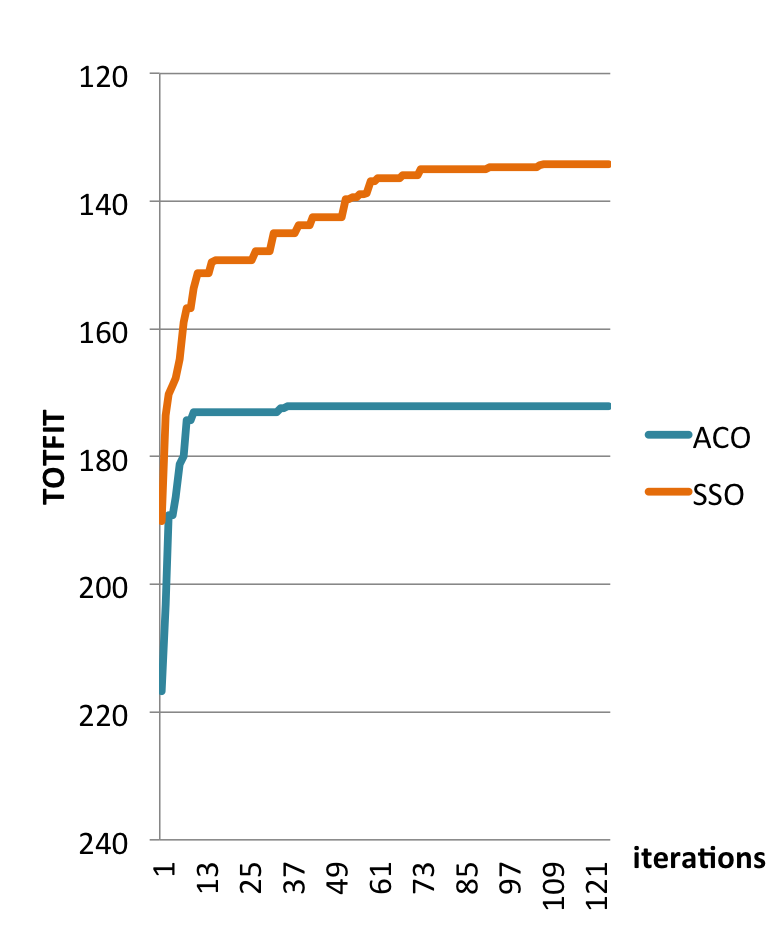
\includegraphics[width=2.5in]{assets/acovsssoNEW.png}
    \end{center}
    \caption{Evolution of TOTFIT for ACO and SSO }
    \label{fig:acovssso} 
\end{figure}
%bytt på att og d0
In Table \vref{table:performanceComparison_4}, the results of the SSO, having four routes, are compared with route sets published in the literature. As one can observe in Table \vref{table:performanceComparison_4}, the route set constructed by SSO has a lower $ATT$ compared to route sets constructed by all other approaches. However, all approaches, except \citep{mandl79, kidwai98, chakroborty02}, produce better route sets concerning the $d_0$ criteria. 

The calculation of $TOTFIT$ is, as mentioned, the sum of $F1$, $F2$ and $F3$. As described in \vref{sec:f1}, a weight parameter, $\sigma$, is used to control the importance of $F1$, $F2$, and $F3$. In the proposed algorithm, $\sigma$ is sat to favor $F1$, which is directly linked to a low $ATT$. Demonstrated in Fig. \vref{fig:mandlWithTT}, when traveling from node 7 to node 14 the algorithm will choose to transfer from route 4 to route 3, and the total travel time will be 20 minutes including a transfer penalty of 5 minutes. $F2$ is concerned whether the algorithm has a high $d_0$, denoting a minimum number of transfers. If $F2$ is favored over $F1$, route 1, which have a direct route from node 7 to node 14, would be selected. The travel time for this route is 27 minutes, increasing the $ATT$. It is worth mentioning that the algorithm does not select $F1$ unconditionally, a high amount of $d_0$ is still important, but the algorithm select the best route set concerning the ratio between the two. 

\begin{figure}[H]
    \begin{center}
    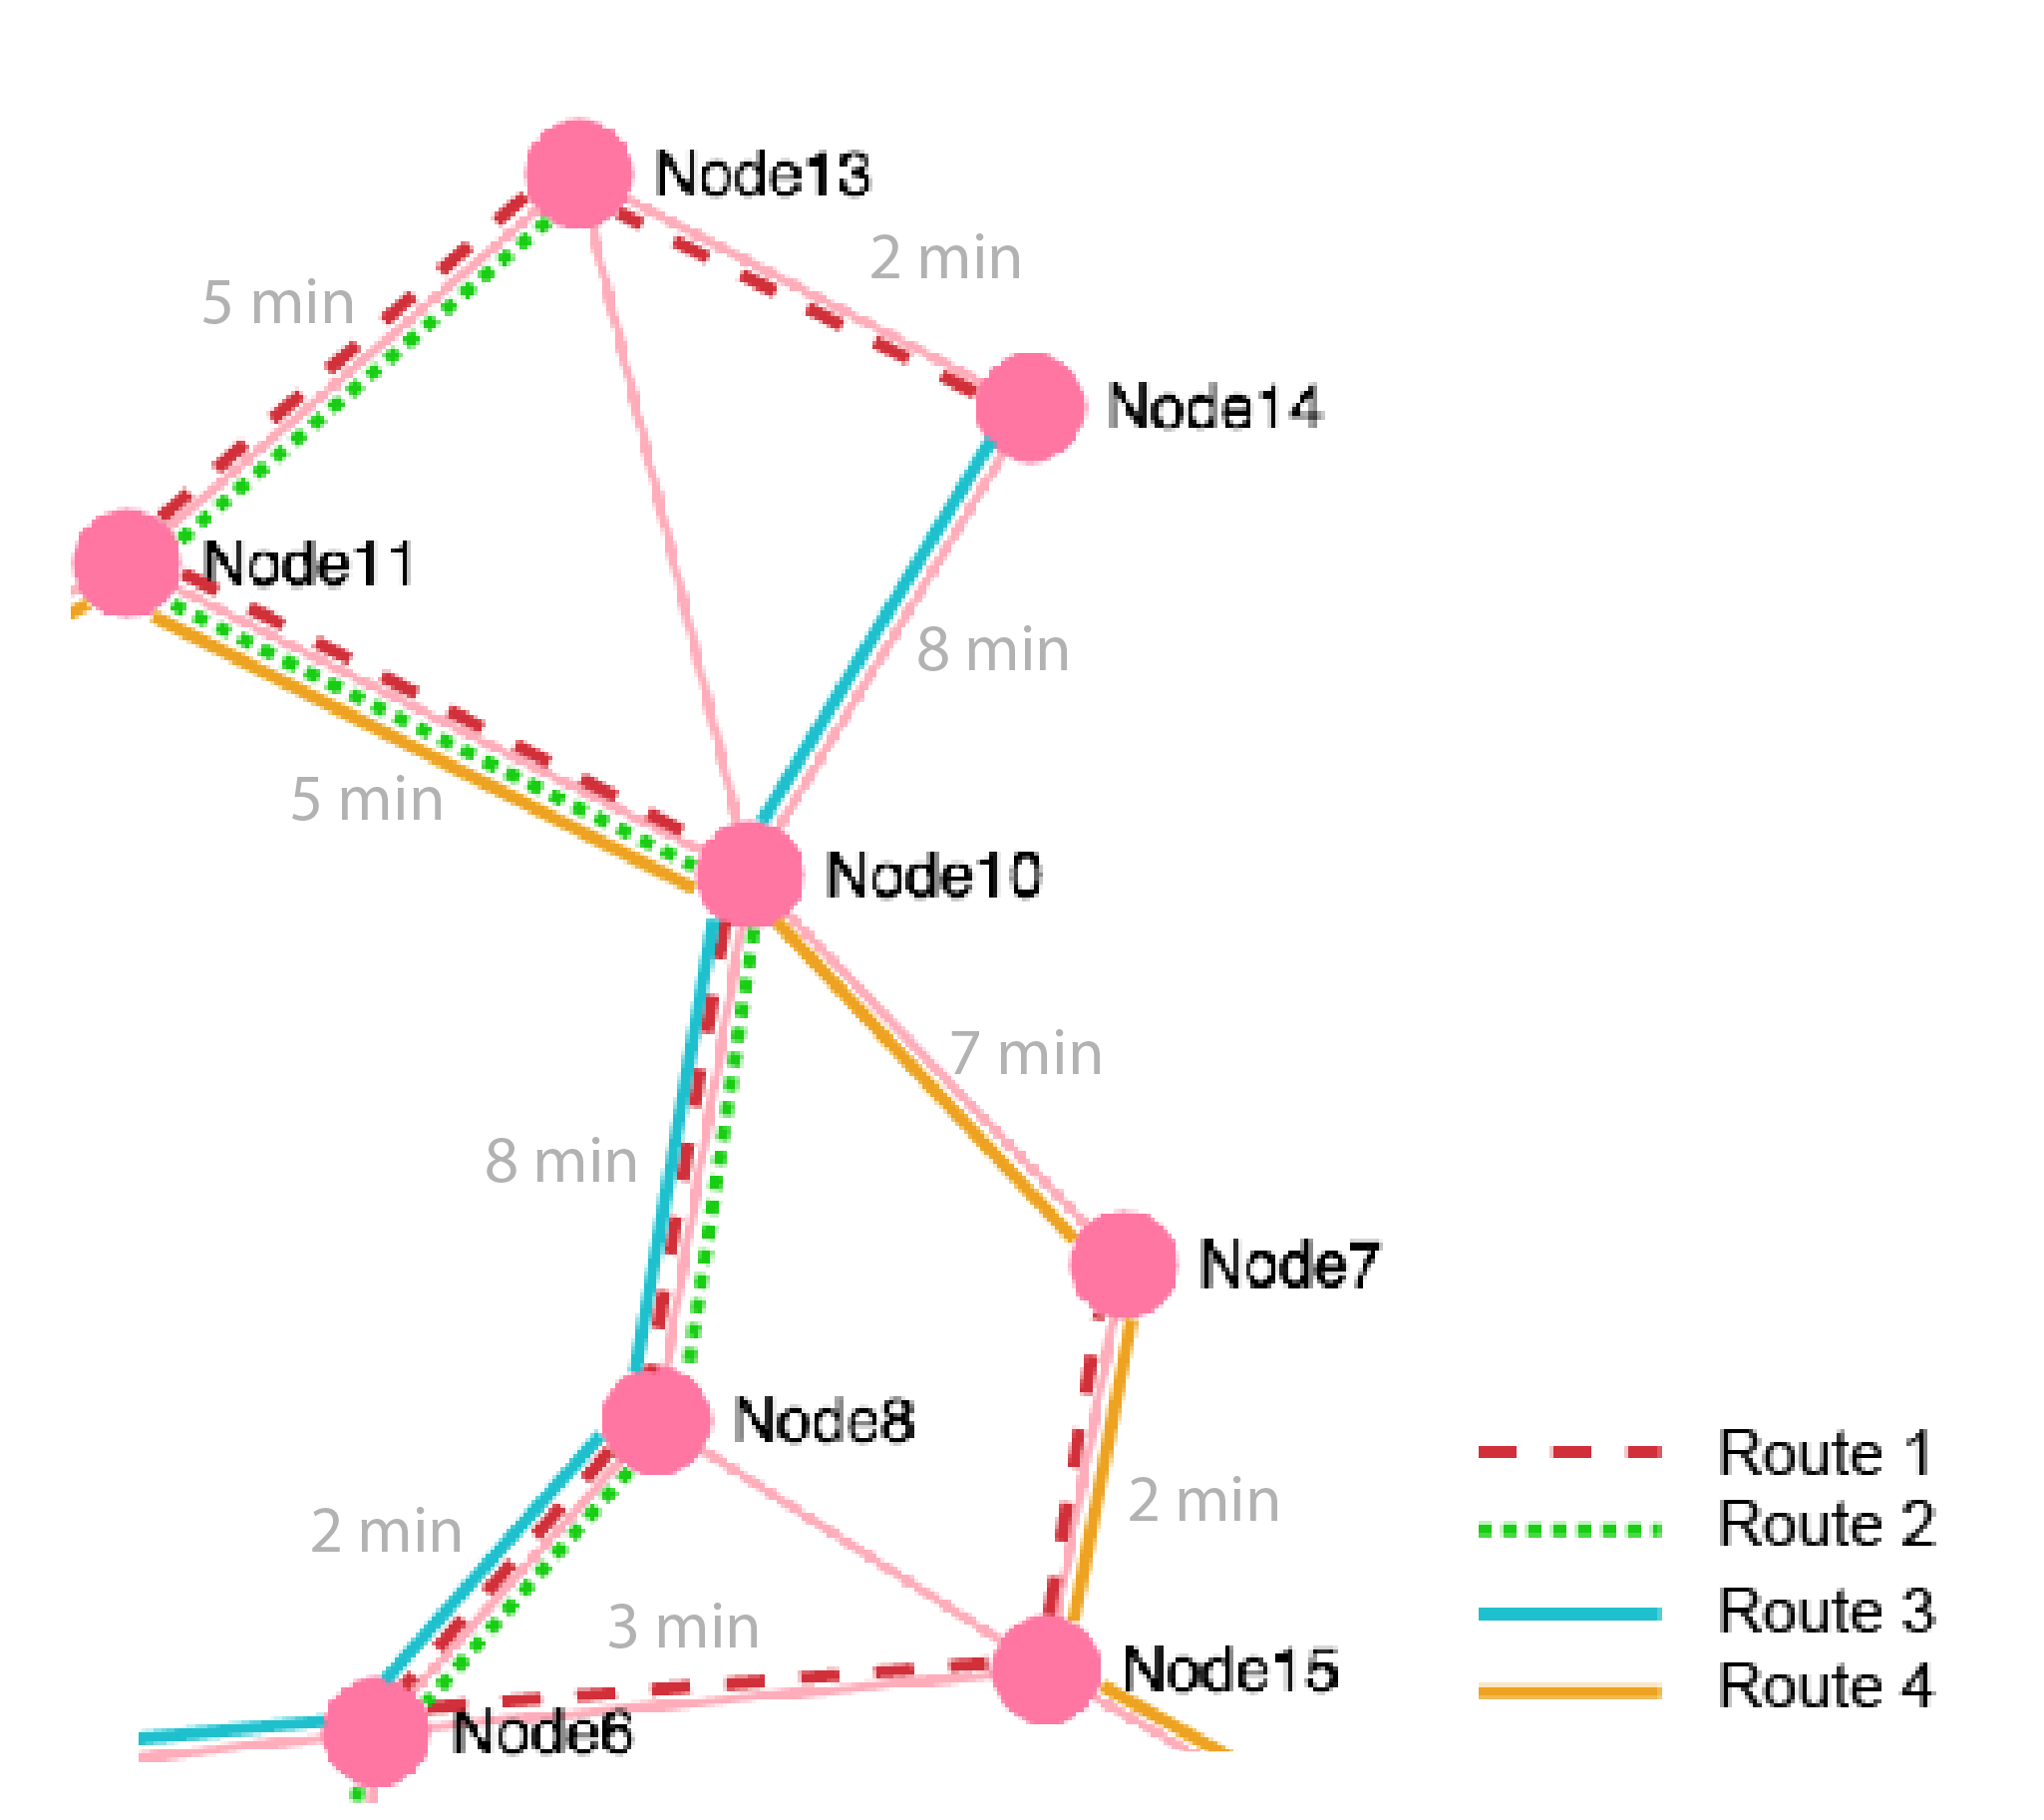
\includegraphics[width=3.5in]{assets/mandl_withTT_utsnitt.png}
    \end{center}
    \caption{A fragment of the best route set, having four route sets, constructed by the proposed algorithm including transfer times in minutes between each node.}
    \label{fig:mandlWithTT} 
\end{figure}

The best route set, having six routes, constructed by the proposed algorithm is presented in Table \vref{table:performanceComparison_bestRouteSet6} and Fig. \vref{fig:bestRouteSet6}. 
Evaluate.

The best route set, having seven routes, constructed by the proposed algorithm is presented in Table \vref{table:performanceComparison_bestRouteSet7} and Fig. \vref{fig:bestRouteSet7}. 
Evaluate

The best route set, having eight routes, constructed by the proposed algorithm is presented in Table \vref{table:performanceComparison_bestRouteSet8} and Fig. \vref{fig:bestRouteSet8}.
Evaluate

As one can observe in \vref{table:performanceComparison_routesets}, the amount of direct travelers increase in line with the number of route sets. This makes sense because thus more route sets the passengers can choose from, thus bigger probability for the passenger finding a convenient route. %However, having eight route sets, it seems to have reached a threshold \emph{\color{blue} TODO: må vente på alle resultater fra sso8}.

 \begin{table}[H]
    \centering
    \begin{tabular}{|l||l|l|l|l|l|}
    \hline
    Route Set & $d_0(\%)$ & $d_1(\%)$ & $d_2(\%)$ & $d_{unsat}(\%)$ & $ATT$ \\
    \hline
    4 & 85.21 & 13.49 & 1.30 & 0.00 & 10.27\\
    6 & 87.17 & 12.0 & 0.82 & 0.01 & 10.11\\
    7 & 88.49 & 10.72 & 0.79 & 0.0 & 10.08\\
    8\\
    \hline
    \end{tabular}
    \caption {Evaluating increase of Route Sets}
    % 50 runs
    \label{table:performanceComparison_routesets}
\end{table}

